% =============================================================================
% Chapter 4: Preparing Training Data
% =============================================================================
\chapter{Preparing Training Data}
\label{ch:preparing-data}

\begin{objectives}
    \item Understand the causal language modeling objective
    \item Learn how input-target pairs are created
    \item Master padding and attention masks
    \item Implement PyTorch Datasets and DataLoaders
    \item Handle batching efficiently
\end{objectives}

% -----------------------------------------------------------------------------
\section{The Language Modeling Objective}
% -----------------------------------------------------------------------------

In \cref{ch:what-are-lms}, we learned that language models predict the next token. But how exactly do we train them to do this? The answer lies in how we structure the training data.

\subsection{Causal Language Modeling}

The training objective for GPT-style models is called \textbf{causal language modeling} (CLM). Given a sequence of tokens, the model learns to predict each token from all preceding tokens.

\begin{definition}[title=Causal Language Modeling]
For a sequence of tokens $(x_1, x_2, \ldots, x_n)$, the model learns to maximize:
\[
\mathcal{L} = \sum_{t=1}^{n} \log P(x_t | x_1, x_2, \ldots, x_{t-1})
\]
This is equivalent to minimizing the \textbf{cross-entropy loss} between predicted and actual tokens.
\end{definition}

The term ``causal'' refers to the constraint that each prediction can only depend on \textit{past} tokens---the model cannot ``peek'' at future tokens.

\subsection{Input and Target Alignment}

To train this objective, we create input-target pairs through a simple \textbf{shift operation}:

\begin{itemize}
    \item \textbf{Input}: All tokens except the last
    \item \textbf{Target}: All tokens except the first
\end{itemize}

\begin{figure}[H]
\centering
\begin{tikzpicture}[
    box/.style={rectangle, draw, minimum width=1.4cm, minimum height=0.7cm, font=\small},
    arrow/.style={-{Stealth[length=2mm]}, thick, gray},
]
    % Original sequence
    \node at (-2, 1.2) {\textbf{Sequence:}};
    \foreach \x/\t in {0/BOS, 1.5/Once, 3/upon, 4.5/a, 6/time, 7.5/EOS} {
        \node[box, fill=blue!10] at (\x, 1.2) {\t};
    }

    % Input (all but last)
    \node at (-2, 0) {\textbf{Input:}};
    \foreach \x/\t in {0/BOS, 1.5/Once, 3/upon, 4.5/a, 6/time} {
        \node[box, fill=green!20] at (\x, 0) {\t};
    }

    % Target (all but first)
    \node at (-2, -1.2) {\textbf{Target:}};
    \foreach \x/\t in {0/Once, 1.5/upon, 3/a, 4.5/time, 6/EOS} {
        \node[box, fill=orange!20] at (\x, -1.2) {\t};
    }

    % Arrows showing prediction
    \foreach \x in {0, 1.5, 3, 4.5, 6} {
        \draw[arrow] (\x, -0.4) -- (\x, -0.8);
    }

    % Labels
    \node[font=\footnotesize, gray] at (0, -1.8) {predict};
    \node[font=\footnotesize, gray] at (6, -1.8) {predict};
\end{tikzpicture}
\caption{The shift operation: input tokens predict the next token as target}
\label{fig:shift-operation}
\end{figure}

For position $i$:
\begin{itemize}
    \item The model sees \texttt{input[0:i+1]} (tokens up to and including position $i$)
    \item It predicts \texttt{target[i]} (the next token)
\end{itemize}

\begin{keypoint}
The model learns from \textbf{every position simultaneously}. A single sequence of $n$ tokens provides $n-1$ training examples (each position predicting the next token).
\end{keypoint}

% -----------------------------------------------------------------------------
\section{The TinyStories Dataset}
% -----------------------------------------------------------------------------

\TryLM trains on TinyStories, available through HuggingFace Datasets.

\subsection{Loading the Dataset}

\begin{lstlisting}[style=python]
from datasets import load_dataset

dataset = load_dataset("roneneldan/TinyStories", split="train")
print(len(dataset))  # ~2.1 million stories
print(dataset[0])
# {'text': 'One day, a little girl named Lily...'}
\end{lstlisting}

\subsection{Dataset Statistics}

\begin{table}[H]
\centering
\begin{tabular}{lr}
\toprule
\textbf{Property} & \textbf{Value} \\
\midrule
Training examples & $\sim$2.1 million \\
Validation examples & $\sim$22,000 \\
Average story length & $\sim$200 words \\
Average tokens (16K vocab) & $\sim$250 tokens \\
\bottomrule
\end{tabular}
\caption{TinyStories dataset statistics}
\end{table}

% -----------------------------------------------------------------------------
\section{Padding and Attention Masks}
% -----------------------------------------------------------------------------

Stories have different lengths. To batch them together efficiently, we need \textbf{padding}.

\subsection{The Padding Problem}

Consider two tokenized sequences:
\begin{lstlisting}[style=shell, numbers=none]
Sequence A: [BOS, Once, upon, a, time, EOS]        # 6 tokens
Sequence B: [BOS, Hi, EOS]                          # 3 tokens
\end{lstlisting}

To form a batch, both must have the same length. We pad the shorter one:
\begin{lstlisting}[style=shell, numbers=none]
Sequence A: [BOS, Once, upon, a, time, EOS]        # 6 tokens
Sequence B: [BOS, Hi, EOS, PAD, PAD, PAD]          # 6 tokens (padded)
\end{lstlisting}

\subsection{Attention Mask}

The \textbf{attention mask} tells the model which positions contain real data:

\begin{lstlisting}[style=shell, numbers=none]
Sequence B input:     [BOS, Hi, EOS, PAD, PAD, PAD]
Attention mask:       [  1,  1,   1,   0,   0,   0]
\end{lstlisting}

\begin{itemize}
    \item \textbf{1}: Real token---include in attention calculations
    \item \textbf{0}: Padding token---ignore in attention
\end{itemize}

\begin{figure}[H]
\centering
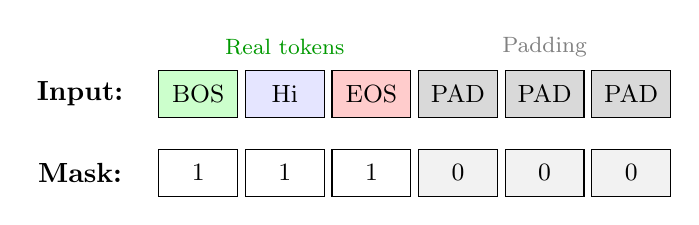
\begin{tikzpicture}[
    box/.style={rectangle, draw, minimum width=1cm, minimum height=0.6cm, font=\small},
]
    % Sequence B
    \node at (-1.5, 1) {\textbf{Input:}};
    \node[box, fill=green!20] at (0, 1) {BOS};
    \node[box, fill=blue!10] at (1.1, 1) {Hi};
    \node[box, fill=red!20] at (2.2, 1) {EOS};
    \node[box, fill=gray!30] at (3.3, 1) {PAD};
    \node[box, fill=gray!30] at (4.4, 1) {PAD};
    \node[box, fill=gray!30] at (5.5, 1) {PAD};

    % Attention mask
    \node at (-1.5, 0) {\textbf{Mask:}};
    \node[box] at (0, 0) {1};
    \node[box] at (1.1, 0) {1};
    \node[box] at (2.2, 0) {1};
    \node[box, fill=gray!10] at (3.3, 0) {0};
    \node[box, fill=gray!10] at (4.4, 0) {0};
    \node[box, fill=gray!10] at (5.5, 0) {0};

    % Labels
    \node[font=\footnotesize, green!60!black] at (1.1, 1.6) {Real tokens};
    \node[font=\footnotesize, gray] at (4.4, 1.6) {Padding};
\end{tikzpicture}
\caption{Attention mask marks real vs. padding tokens}
\label{fig:attention-mask}
\end{figure}

\subsection{Labels and the -100 Convention}

For labels (targets), we use a special convention: \textbf{-100 marks positions to ignore in the loss}.

\begin{lstlisting}[style=shell, numbers=none]
Input:   [BOS, Hi, PAD, PAD, PAD]
Labels:  [ Hi, EOS, -100, -100, -100]
\end{lstlisting}

PyTorch's \texttt{cross\_entropy} function automatically ignores positions with label -100:

\begin{lstlisting}[style=python]
import torch.nn.functional as F

# -100 positions are ignored in loss calculation
loss = F.cross_entropy(
    logits.view(-1, vocab_size),
    labels.view(-1),
    ignore_index=-100  # This is the default
)
\end{lstlisting}

\begin{keypoint}
Using -100 for padding labels ensures the model isn't penalized for predictions at padding positions---it only learns from real tokens.
\end{keypoint}

% -----------------------------------------------------------------------------
\section{The TryLM Dataset Implementation}
% -----------------------------------------------------------------------------

Let's examine how \TryLM implements the dataset.

\subsection{Dataset Class}

\begin{lstlisting}[style=python, caption={TinyStoriesDataset from data.py}]
class TinyStoriesDataset(Dataset):
    def __init__(
        self,
        tokenizer: TryLMTokenizer,
        split: str = "train",
        context_length: int = 512,
        dataset_name: str = "roneneldan/TinyStories",
    ) -> None:
        self.tokenizer = tokenizer
        self.context_length = context_length

        # Load dataset
        dataset = load_dataset(dataset_name, split=split)

        # Tokenize all texts upfront
        self.token_ids: list[list[int]] = []
        for item in dataset:
            ids = tokenizer.encode(item["text"], add_special_tokens=True)
            if len(ids) >= 2:  # Need at least 2 tokens
                self.token_ids.append(ids)

    def __len__(self) -> int:
        return len(self.token_ids)
\end{lstlisting}

\subsection{The \texttt{\_\_getitem\_\_} Method}

This is where the magic happens---creating input-target pairs:

\begin{lstlisting}[style=python, caption={Creating input-target pairs}]
def __getitem__(self, idx: int) -> dict[str, torch.Tensor]:
    ids = self.token_ids[idx]

    # Truncate if too long
    if len(ids) > self.context_length + 1:
        ids = ids[: self.context_length + 1]

    # Split into input and target (the shift operation!)
    input_ids = ids[:-1]   # All but last
    labels = ids[1:]       # All but first

    # Pad to context_length
    pad_len = self.context_length - len(input_ids)
    attention_mask = [1] * len(input_ids) + [0] * pad_len

    input_ids = input_ids + [self.tokenizer.pad_id] * pad_len
    labels = labels + [-100] * pad_len  # -100 ignored in loss

    return {
        "input_ids": torch.tensor(input_ids, dtype=torch.long),
        "labels": torch.tensor(labels, dtype=torch.long),
        "attention_mask": torch.tensor(attention_mask, dtype=torch.long),
    }
\end{lstlisting}

\subsection{Step-by-Step Example}

Let's trace through a concrete example:

\begin{lstlisting}[style=python]
# Original tokenized story (8 tokens)
ids = [1, 4521, 2378, 263, 1159, 267, 5831, 2]
#     BOS Once  upon  a    time  ,    .     EOS

# Context length = 6 (for this example)
# Need context_length + 1 = 7 tokens
# 8 > 7, so truncate:
ids = ids[:7]  # [1, 4521, 2378, 263, 1159, 267, 5831]

# Shift operation:
input_ids = ids[:-1]  # [1, 4521, 2378, 263, 1159, 267]
labels = ids[1:]      # [4521, 2378, 263, 1159, 267, 5831]

# Pad to context_length (6)
# Already length 6, so no padding needed
attention_mask = [1, 1, 1, 1, 1, 1]
\end{lstlisting}

For a shorter sequence:
\begin{lstlisting}[style=python]
# Short story (4 tokens)
ids = [1, 487, 5831, 2]  # BOS Hi . EOS

# Shift operation:
input_ids = [1, 487, 5831]     # BOS Hi .
labels = [487, 5831, 2]        # Hi . EOS

# Pad to context_length (6)
pad_len = 6 - 3 = 3

attention_mask = [1, 1, 1, 0, 0, 0]
input_ids = [1, 487, 5831, PAD, PAD, PAD]
labels = [487, 5831, 2, -100, -100, -100]
\end{lstlisting}

% -----------------------------------------------------------------------------
\section{DataLoaders and Batching}
% -----------------------------------------------------------------------------

PyTorch's \texttt{DataLoader} handles batching, shuffling, and parallel data loading.

\subsection{Creating DataLoaders}

\begin{lstlisting}[style=python, caption={DataLoader creation from data.py}]
def create_dataloaders(
    tokenizer: TryLMTokenizer,
    model_config: ModelConfig,
    train_config: TrainConfig,
) -> tuple[DataLoader, DataLoader]:

    train_dataset = TinyStoriesDataset(
        tokenizer=tokenizer,
        split=train_config.train_split,
        context_length=model_config.context_length,
    )

    train_loader = DataLoader(
        train_dataset,
        batch_size=train_config.batch_size,  # e.g., 64
        shuffle=True,          # Randomize order each epoch
        num_workers=4,         # Parallel data loading
        pin_memory=True,       # Faster GPU transfer
        drop_last=True,        # Drop incomplete final batch
    )

    return train_loader, val_loader
\end{lstlisting}

\subsection{Batch Structure}

Each batch is a dictionary of tensors:

\begin{lstlisting}[style=python]
batch = next(iter(train_loader))

print(batch["input_ids"].shape)      # [64, 512] - batch_size x context_length
print(batch["labels"].shape)         # [64, 512]
print(batch["attention_mask"].shape) # [64, 512]
\end{lstlisting}

\begin{figure}[H]
\centering
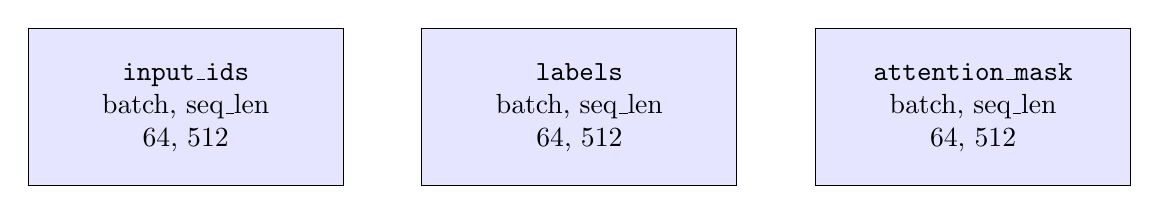
\begin{tikzpicture}[
    tensor/.style={rectangle, draw, minimum width=4cm, minimum height=2cm, fill=blue!10},
]
    \node[tensor] (input) at (0, 0) {
        \begin{tabular}{c}
        \texttt{input\_ids} \\
        \shape{batch, seq\_len} \\
        \shape{64, 512}
        \end{tabular}
    };

    \node[tensor] (labels) at (5, 0) {
        \begin{tabular}{c}
        \texttt{labels} \\
        \shape{batch, seq\_len} \\
        \shape{64, 512}
        \end{tabular}
    };

    \node[tensor] (mask) at (10, 0) {
        \begin{tabular}{c}
        \texttt{attention\_mask} \\
        \shape{batch, seq\_len} \\
        \shape{64, 512}
        \end{tabular}
    };
\end{tikzpicture}
\caption{Batch tensor shapes for batch size 64 and context length 512}
\label{fig:batch-shapes}
\end{figure}

\subsection{DataLoader Parameters Explained}

\begin{table}[H]
\centering
\begin{tabular}{lp{8cm}}
\toprule
\textbf{Parameter} & \textbf{Purpose} \\
\midrule
\texttt{batch\_size} & Number of sequences per batch (64 default) \\
\texttt{shuffle} & Randomize order each epoch (True for training) \\
\texttt{num\_workers} & Parallel processes for data loading \\
\texttt{pin\_memory} & Pre-allocate GPU memory for faster transfer \\
\texttt{drop\_last} & Drop incomplete final batch (for consistent batch sizes) \\
\bottomrule
\end{tabular}
\caption{DataLoader configuration parameters}
\end{table}

% -----------------------------------------------------------------------------
\section{Streaming Datasets}
% -----------------------------------------------------------------------------

For very large datasets, loading everything into memory may be impractical. \TryLM supports \textbf{streaming} datasets.

\subsection{Memory Comparison}

\begin{table}[H]
\centering
\begin{tabular}{lll}
\toprule
\textbf{Approach} & \textbf{Memory Usage} & \textbf{Use Case} \\
\midrule
Standard Dataset & High (all data in RAM) & Small-medium datasets \\
Streaming Dataset & Low (one batch at a time) & Large datasets \\
\bottomrule
\end{tabular}
\caption{Standard vs. streaming dataset comparison}
\end{table}

\subsection{Streaming Implementation}

\begin{lstlisting}[style=python, caption={StreamingTinyStoriesDataset from data.py}]
class StreamingTinyStoriesDataset(IterableDataset):
    def __iter__(self) -> Iterator[dict[str, torch.Tensor]]:
        dataset = load_dataset(
            self.dataset_name,
            split=self.split,
            streaming=True,  # Key difference!
        )

        if self.shuffle:
            dataset = dataset.shuffle(seed=self.seed, buffer_size=10000)

        for item in dataset:
            ids = self.tokenizer.encode(item["text"])
            # ... same processing as standard dataset
            yield {
                "input_ids": torch.tensor(input_ids),
                "labels": torch.tensor(labels),
                "attention_mask": torch.tensor(attention_mask),
            }
\end{lstlisting}

The streaming dataset loads and processes data on-the-fly, never holding the entire dataset in memory.

% -----------------------------------------------------------------------------
\section{Context Windows and Truncation}
% -----------------------------------------------------------------------------

\subsection{Why Truncate?}

The model has a fixed \textbf{context length} (512 tokens by default). Sequences longer than this must be truncated.

\begin{lstlisting}[style=python]
# If sequence is too long, truncate
if len(ids) > self.context_length + 1:
    ids = ids[: self.context_length + 1]
\end{lstlisting}

The ``+1'' accounts for the shift operation---we need \texttt{context\_length} tokens for input plus one more for the final target.

\subsection{Alternative: Chunking}

Instead of truncating long sequences, you could chunk them:

\begin{lstlisting}[style=python]
# Split long sequence into multiple training examples
def chunk_sequence(ids, context_length):
    chunks = []
    for i in range(0, len(ids) - 1, context_length):
        chunk = ids[i : i + context_length + 1]
        if len(chunk) >= 2:
            chunks.append(chunk)
    return chunks
\end{lstlisting}

\TryLM uses simple truncation, but chunking can be more data-efficient for long documents.

% -----------------------------------------------------------------------------
\section{Data Flow Summary}
% -----------------------------------------------------------------------------

\begin{figure}[H]
\centering
\begin{tikzpicture}[
    box/.style={rectangle, draw, rounded corners, minimum width=3.5cm, minimum height=0.8cm, align=center, fill=blue!10},
    arrow/.style={-{Stealth[length=2mm]}, thick},
    data/.style={font=\footnotesize\ttfamily, gray},
]
    % Boxes
    \node[box] (raw) at (0, 0) {Raw Text};
    \node[box] (tok) at (0, -1.5) {Tokenizer};
    \node[box] (ids) at (0, -3) {Token IDs};
    \node[box] (shift) at (0, -4.5) {Shift \& Pad};
    \node[box] (batch) at (0, -6) {Batch Tensors};
    \node[box] (model) at (0, -7.5) {Model};

    % Arrows
    \draw[arrow] (raw) -- (tok);
    \draw[arrow] (tok) -- (ids);
    \draw[arrow] (ids) -- (shift);
    \draw[arrow] (shift) -- (batch);
    \draw[arrow] (batch) -- (model);

    % Data annotations
    \node[data, right=0.5cm of raw] {``Once upon a time''};
    \node[data, right=0.5cm of ids] {[1, 4521, 2378, 263, 1159, 2]};
    \node[data, right=0.5cm of shift] {input, labels, mask};
    \node[data, right=0.5cm of batch] {\shape{batch, seq\_len}};
\end{tikzpicture}
\caption{Complete data pipeline from raw text to model input}
\label{fig:data-pipeline}
\end{figure}

% -----------------------------------------------------------------------------
\section{Common Pitfalls}
% -----------------------------------------------------------------------------

\begin{pitfall}[title=Off-by-One Errors]
The shift operation requires careful indexing:
\begin{lstlisting}[style=python]
# WRONG: input and labels have different lengths
input_ids = ids[:-1]  # n-1 tokens
labels = ids           # n tokens (mismatch!)

# CORRECT: same length, offset by 1
input_ids = ids[:-1]  # n-1 tokens
labels = ids[1:]      # n-1 tokens
\end{lstlisting}
\end{pitfall}

\begin{pitfall}[title=Forgetting -100 for Padding]
If you pad labels with 0 instead of -100, the model will try to predict the padding token:
\begin{lstlisting}[style=python]
# WRONG: model learns to predict padding tokens
labels = labels + [0] * pad_len

# CORRECT: padding positions ignored in loss
labels = labels + [-100] * pad_len
\end{lstlisting}
\end{pitfall}

\begin{pitfall}[title=Inconsistent Context Length]
The dataset must use the same context length as the model:
\begin{lstlisting}[style=python]
# These must match!
dataset = TinyStoriesDataset(context_length=512, ...)
model = GPT(ModelConfig(context_length=512))
\end{lstlisting}
\end{pitfall}

% -----------------------------------------------------------------------------
\section{Exercises}
% -----------------------------------------------------------------------------

\begin{exercise}
\textbf{Trace the Shift Operation}

Given the token sequence \texttt{[1, 100, 200, 300, 2]} with context length 4:
\begin{enumerate}
    \item What are \texttt{input\_ids}?
    \item What are \texttt{labels}?
    \item What is the \texttt{attention\_mask}?
\end{enumerate}
\end{exercise}

\begin{exercise}
\textbf{Visualize a Batch}

Load the dataset and examine a real batch:
\begin{lstlisting}[style=python, numbers=none]
from trylm.data import create_dataloaders
from trylm.tokenizer import TryLMTokenizer
from trylm.config import ModelConfig, TrainConfig

tokenizer = TryLMTokenizer.load("data/tokenizer")
train_loader, _ = create_dataloaders(
    tokenizer, ModelConfig(), TrainConfig()
)

batch = next(iter(train_loader))
print("Shapes:", {k: v.shape for k, v in batch.items()})
print("First sequence input:", batch["input_ids"][0][:20])
print("First sequence labels:", batch["labels"][0][:20])
\end{lstlisting}
\end{exercise}

\begin{exercise}
\textbf{Count Tokens}

Calculate the total number of tokens in the training set:
\begin{lstlisting}[style=python, numbers=none]
total_tokens = 0
for batch in train_loader:
    mask = batch["attention_mask"]
    total_tokens += mask.sum().item()
print(f"Total tokens: {total_tokens:,}")
\end{lstlisting}

How does this compare to the theoretical maximum (num\_examples $\times$ context\_length)?
\end{exercise}

% -----------------------------------------------------------------------------
\section{Summary}
% -----------------------------------------------------------------------------

\begin{summary}
    \item \textbf{Causal language modeling} trains models to predict the next token
    \item The \textbf{shift operation} creates input-target pairs: \texttt{input = ids[:-1]}, \texttt{target = ids[1:]}
    \item \textbf{Padding} equalizes sequence lengths for batching
    \item \textbf{Attention masks} mark real vs. padding tokens (1 vs. 0)
    \item \textbf{-100 in labels} tells PyTorch to ignore padding positions in the loss
    \item \textbf{DataLoaders} handle batching, shuffling, and parallel loading
    \item \textbf{Streaming datasets} reduce memory usage for large datasets
\end{summary}

We now have all the pieces to feed data into our model. In the next chapter, we'll begin building the model itself, starting with how token IDs become continuous vector embeddings.
